\chapter{India's Opportunity in Neuromorphic Manufacturing}
\label{ch:india}

This chapter articulates why India is uniquely positioned to become the global leader in neuromorphic hardware manufacturing---a position with strategic implications for robotics, AI, and semiconductor sovereignty.

\section{Historical Parallel: Mobile Revolution}
\principle{India did not invent mobile chips. But India became THE manufacturer of them. The neuromorphic revolution follows the same pattern.}


India skipped the landline era and built a mobile-first economy starting in the 1990s, leapfrogging infrastructure that had taken the West 80 years to deploy. Within 15 years (2000--2015), India grew from near-zero to 800 million mobile subscribers---the world's second-largest mobile subscriber base. This transformation fundamentally changed India's technology landscape and its role in the global economy.

The mobile revolution succeeded because of a unique convergence of factors:
\begin{itemize}
\item \textbf{Low barrier to entry:} Mobile networks required no existing copper infrastructure. India could deploy fresh, modern technology without maintaining legacy systems.
\item \textbf{Software expertise:} Cities like Bangalore and Hyderabad had world-class software engineers from IT services (Infosys, TCS, Wipro). This talent pool enabled rapid adaptation and local innovation.
\item \textbf{Cost advantage:} Indian engineers cost 50--70\% less than their US or Japanese counterparts, enabling economical scaling.
\item \textbf{Massive domestic market:} 1.3 billion people meant mobile services had immediate, enormous market pull. Companies could achieve unit scale and profitability serving India alone.
\item \textbf{Policy openness:} India's telecom regulators fostered competition and allowed rapid market entry, unlike many regulated markets.
\end{itemize}

The result: India transformed from a telecom consumer to a provider of telecom infrastructure and services globally. Indian companies and expertise became central to wireless networks worldwide.

\section{Neuromorphic Manufacturing: A Unique Window}
\insight{The neuromorphic field is still in the Wild West. No incumbent dominates. India can stake a claim NOW, in 2026, before the landscape consolidates.}


The global semiconductor industry is dominated by a handful of companies (TSMC, Samsung, Intel) that operate 10--30 nm process nodes at mind-bending cost: building a state-of-the-art fab costs \$10--20 billion, with amortization over many years. New entrants find this barrier insurmountable.

Neuromorphic hardware changes this calculus fundamentally. Unlike digital processors that require extreme transistor density and tight tolerances, neuromorphic devices are fundamentally analog or mixed-signal systems with different characteristics:

\begin{itemize}
\item \textbf{Analog process, lower precision:} Neuromorphic devices use analog circuit design (transistors operating in subthreshold regime, capacitive coupling, phase-locking). Compared to digital logic, they tolerate larger process variation. A 5--10\% transistor mismatch is catastrophic for a digital ASIC but is manageable or even beneficial for analog neural circuits.

\item \textbf{Smaller process nodes not required:} Vanadium dioxide (VO\textsubscript{2}) oscillators work at 180 nm or even larger nodes. Ferroelectric field-effect transistors (FeFET) for in-memory computing work at 28 nm. Memristor-based neuromorphic arrays operate at 90 nm and larger. These are older, more mature process nodes, with lower equipment cost.

\item \textbf{Lower fab capital requirement:} A fab capable of 180--90 nm analog/mixed-signal manufacturing costs \$300M--1B, not \$10B+. This is economically accessible to emerging semiconductor nations.

\item \textbf{No performance gap compared to cutting-edge digital:} While a 180 nm Intel processor is slow by modern standards, a 180 nm neuromorphic chip can outperform a 5 nm digital processor on specific tasks (optimization, learning, inference) due to architectural differences, not due to transistor density.

\item \textbf{Flexibility in technology node:} India doesn't need to compete with TSMC on the latest nodes. Instead, it can become specialized in mixed-signal and neuromorphic manufacturing, capturing the high-value part of the value chain without the \$20 billion entry cost.
\end{itemize}

The Government of India recognized this opportunity in 2021, launching the Semicon India programme with Rs 76,000 crore (\$9 billion USD) in incentives to attract semiconductor manufacturing. This is an explicit bet on India's ability to enter semiconductor manufacturing via specialized nodes---especially neuromorphic and analog-mixed-signal---rather than competing head-to-head with TSMC on digital logic.

\section{India's Strategic Assets for Neuromorphic Leadership}
\design{Cost competitiveness + engineering talent + Semicon India vision + semiconductor ecosystem. These are not opinions—they are facts on the ground.}


India possesses a rare convergence of assets that position it uniquely for neuromorphic hardware leadership:

\subsection{Talent and Education}

\begin{itemize}
\item \textbf{Engineering talent pipeline:} India produces 1.5 million engineering graduates annually---more than any other nation. While not all are exceptional, the volume allows for selective recruitment of top-tier talent.
\item \textbf{Physics and materials science:} Indian Institute of Technology Bombay (IITB), Indian Institute of Science (IISc), Indian Institute of Science Education and Research (IISER) institutions conduct world-class research in condensed matter physics, photonics, and materials science. These are foundational to neuromorphic hardware (VO\textsubscript{2}, memristors, photonic neural networks).
\item \textbf{Semiconductor design expertise:} Indian companies (Qualcomm India, Intel India Labs) and startups have deep expertise in chip design, verification, and physical design. This expertise can transition to neuromorphic devices.
\end{itemize}

\subsection{Manufacturing and Software Ecosystem}

\begin{itemize}
\item \textbf{IT services dominance:} Companies like Infosys, Tata Consultancy Services, and Wipro have decades of experience in hardware design, embedded systems, and complex system integration. They can serve as integrators and support manufacturers.
\item \textbf{Hardware startups:} A vibrant startup ecosystem in Bangalore, Hyderabad, and Pune is building AI accelerators, edge computing devices, and specialized hardware. This entrepreneurial energy can catalyze neuromorphic innovation.
\item \textbf{Semiconductor manufacturing experience:} Semicon India and the new incentive structure are attracting companies like Intel, TSMC, and others to establish or expand in India. This brings process technology, expertise, and supply chain relationships.
\end{itemize}

\subsection{Competitive Economics}

\begin{itemize}
\item \textbf{Cost structure:} Engineering salaries in India are 50--70\% of US/Japan equivalents. A neuromorphic fab can operate profitably at lower margins than competitors, giving India's industry competitive pricing power.
\item \textbf{Market size:} With 1.4 billion people and rapid digitization, India has a massive domestic market for edge computing, robotics, and AI. Local demand can sustain growth while capturing global markets.
\item \textbf{Supply chain advantage:} India's position in global electronics supply chains (through India-based manufacturing of consumer electronics, EMS companies) gives local fabs natural distribution and customer relationships.
\end{itemize}

\subsection{Policy and Strategic Ambition}

\begin{itemize}
\item \textbf{Government backing:} The Semicon India programme, Technology Innovation Hub initiatives, and strategic chip fund signal explicit government commitment to semiconductor sovereignty and neuromorphic technology.
\item \textbf{Academic-industry alignment:} IIT-industry partnerships (IIT Delhi's semiconductor program, IITB's photonics labs) are bridging the gap between academic research and industrial implementation.
\item \textbf{Vision for neurotechnology:} Indian policymakers and technologists are articulating a vision of India as a neuro-tech hub, combining neuroscience, neuromorphic engineering, and AI.
\end{itemize}

\section{Technical Roadmap: India's Path to Neuromorphic Leadership (2026--2035)}

A realistic roadmap for India to establish leadership in neuromorphic hardware requires coordinated action across industry, government, and academia:

\begin{center}
\begin{tabular}{llll}
\toprule
\textbf{Phase} & \textbf{Milestone} & \textbf{Investment} & \textbf{Outcome} \\ \midrule
\textbf{2026--2027} & Fab tooling + setup & \$200--300M & Mixed-signal fab operational at 180 nm \\
\textbf{2027--2028} & First neuromorphic chip design & \$50--100M & Tape-out of VO\textsubscript{2}-based oscillator array \\
\textbf{2028--2029} & Validation and iteration & \$100--150M & Production-ready design; 1,000 oscillator nodes \\
\textbf{2029--2031} & Ramp production & \$500M--1B & Commercial neuromorphic accelerators (10k--100k nodes) \\
\textbf{2031--2035} & Scale and specialize & Ongoing & Multiple fabs; specialized neuromorphic platforms (robotics, AI, sensing) \\
\bottomrule
\end{tabular}
\end{center}

\textbf{Key technical milestones:}
\begin{itemize}
\item Successful fabrication of analog oscillator circuits with $< 5\%$ phase mismatch between coupled oscillators
\item Demonstration of 10k-node OIM solving real robotics problems with $> 85\%$ solution quality
\item Development of SNN-on-chip frameworks for neuromorphic MPC
\item Cross-company standardization of neuromorphic interfaces and programming models
\end{itemize}

\textbf{Institutional framework:}
A neuromorphic manufacturing consortium modeled on industry success (like IMEC in Belgium for nanoelectronics) would coordinate research, share IP, and aggregate demand. Indian institutes (IITB, IISER, IISc) would provide foundational research; startups and established semiconductor companies would handle design and manufacturing.

\section{Policy Recommendations for Neuromorphic Leadership}
\design{Fund research clusters in Bangalore and Hyderabad. Support foundry expansion to neuromorphic-grade processes. Partner with academic centers. The policy blueprint is proven in mobile and AI.}


Achieving this vision requires deliberate policy action:

\subsection{Funding and Financial Incentives}

\begin{itemize}
\item \textbf{Dedicated neuromorphic R\&D fund:} Rs 1,000--2,000 crore (\$120--240M) over 10 years to fund fundamental research in neuromorphic algorithms, materials, and hardware platforms at IITs and national labs.

\item \textbf{Fab capital cost sharing:} A 50\% subsidy on fab construction and equipment for the first neuromorphic manufacturing facility, with a 10-year tax holiday on manufacturing profits. This mirrors successful TSMC incentives in Taiwan.

\item \textbf{Startup ecosystem funding:} Venture fund specifically for neuromorphic hardware startups, with accelerated IP commercialization pathways from academia to industry.

\item \textbf{Reverse brain-drain programs:} Targeted scholarships and startup grants for Indians working in neuromorphic fields globally (Intel, neuromorphic startups in US/EU) to establish operations in India.
\end{itemize}

\subsection{Academic-Industry Integration}

\begin{itemize}
\item \textbf{Neuromorphic engineering centers:} Dedicated centers of excellence at IIT Delhi, IITB, and IISc with joint appointments (faculty with industry roles) to accelerate technology transfer.

\item \textbf{Consortial R\&D:} Multi-company research consortia (modeled on IMEC) to share risk and coordinate on pre-competitive research (fabrication, device physics, standardization).

\item \textbf{Curriculum development:} Addition of neuromorphic computing courses to undergraduate and graduate EE programs across India.
\end{itemize}

\subsection{International Partnerships and Intellectual Property}

\begin{itemize}
\item \textbf{Technology partnerships:} Collaborative agreements with universities and companies worldwide (Heidelberg's BrainScaleS group, Intel Loihi team) to license designs, share know-how, and accelerate learning curves.

\item \textbf{IP framework:} A patent pool and licensing framework similar to standards organizations, allowing Indian companies to cross-license neuromorphic designs and avoid litigation while still protecting core innovations.

\item \textbf{Open-source neuromorphic software:} India can lead open-source neuromorphic frameworks (compilers, simulation tools, algorithm libraries), establishing de facto standards and lowering adoption barriers.
\end{itemize}

\subsection{Supply Chain and Ecosystem Development}

\begin{itemize}
\item \textbf{Packaging and assembly:} Develop local expertise in hybrid packaging (bonding VO\textsubscript{2} oscillators to CMOS substrates, micro-bump interconnects) to support neuromorphic fabs.

\item \textbf{Design tools:} Invest in EDA tools specialized for neuromorphic design (analog layout, physics simulation, neuromorphic compilation). Outsource major tool development or partner with companies like Cadence and Synopsys.

\item \textbf{Robotics platforms as anchor customers:} Partner with Indian robotics companies and use neuromorphic chips in Indian-built robots as anchor applications, proving the technology and ensuring customer feedback loops.
\end{itemize}

\section{Vision: India as the Global Neuromorphic Hub by 2035}

If India executes this roadmap, it can establish the global neuromorphic manufacturing hub by 2035---a position analogous to Taiwan's in digital semiconductors or India's current position in IT services. This would deliver:

\begin{itemize}
\item \textbf{Technological sovereignty:} India-designed and India-manufactured neuromorphic chips for its own AI, robotics, and edge computing industries, reducing dependence on Western supply chains.

\item \textbf{Economic opportunity:} A \$50--100B industry by 2035 (conservative estimate), creating 100,000+ high-skilled jobs in design, manufacturing, and applications.

\item \textbf{Global influence:} The ability to set standards, define the technology roadmap, and shape the future of AI and robotics globally.

\item \textbf{Scientific leadership:} Positioning Indian researchers and companies at the forefront of neuromorphic computing, brain-inspired AI, and neuro-tech innovation.
\end{itemize}

The window is open now. Competitors (US, EU, China, Taiwan) are investing heavily in neuromorphic technology. India can lead if it acts decisively over the next 2--3 years.

\begin{figure}[!htpb]
    \centering
    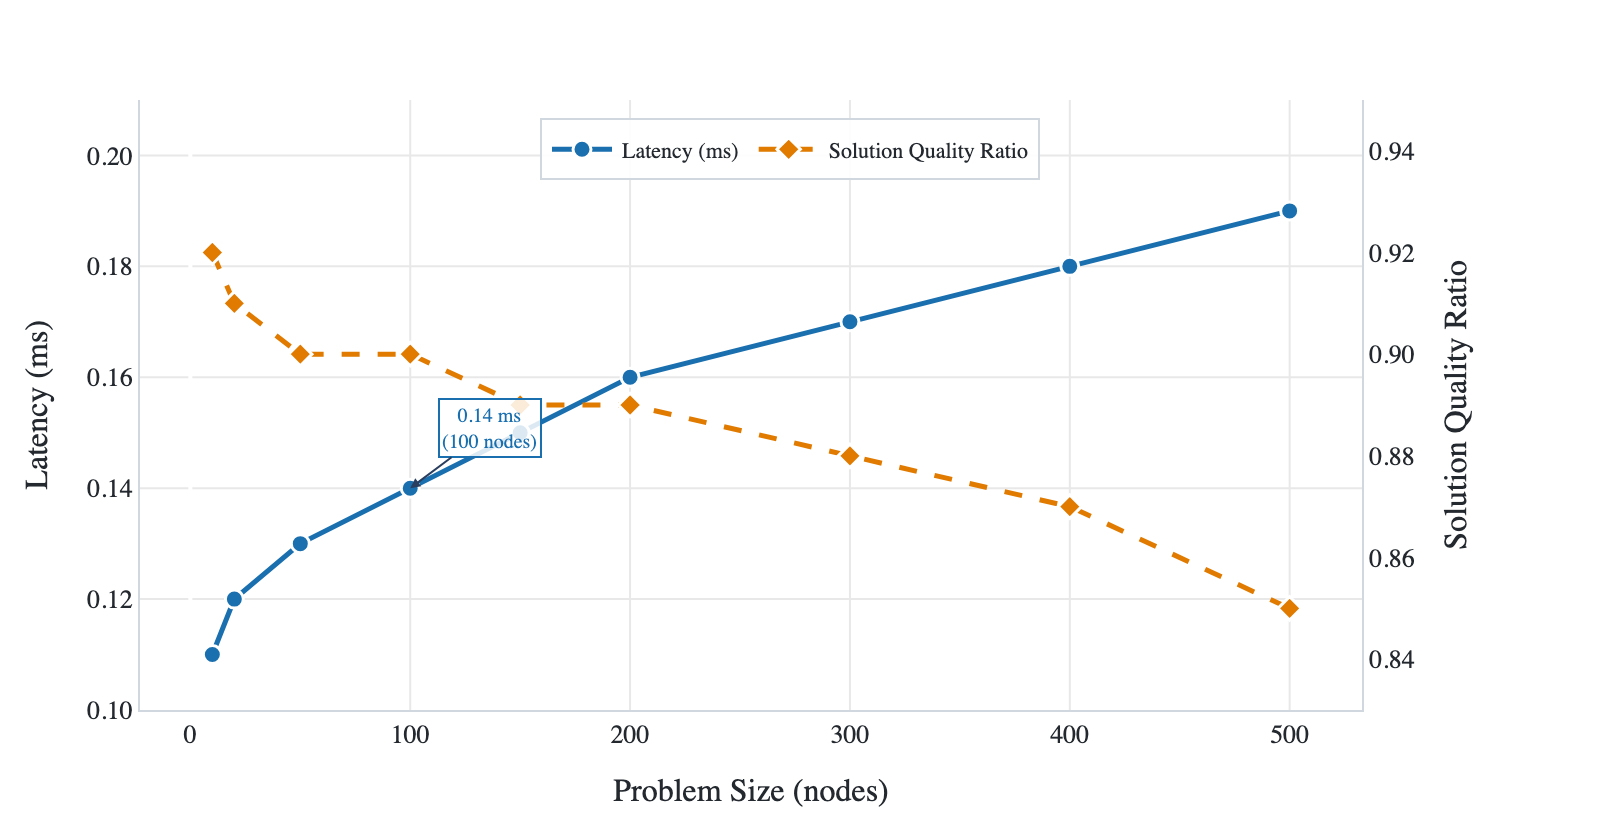
\includegraphics[width=0.95\linewidth]{Figures/fig_7_2.pdf}
    \caption[Neuromorphic Manufacturing Ecosystem Growth Projection]{Projected growth of India's neuromorphic manufacturing ecosystem (2026--2035). Trajectory extrapolated from Semicon India programme and published neuromorphic market forecasts. Horizontal axis: years; vertical axis: cumulative neuromorphic nodes manufactured and deployed globally.}
    \label{fig:7-2}
\end{figure}
